\subsection{Requirements}\label{sec:requirements}

\newcounter{req_count}

\subsubsection{Automation}

\stepcounter{req_count}

%Finally, also considering the multiplicity of edge servers and the need for a scalable solution for the provisioning of edge infrastructure as a service, the following requirement have been defined:
TODO: introduce the need for automation, possibly linking to serverless computing.
\textcolor{blue}{Martin's comment: I've added the following paragraph linked with what is said about serverless+automation. Please check.}

In order to materialize the computational continuum, it is crucial to detach the control and management of the infrastructure from the application developer. The model should be automated and transparent, where the developer is unaware of which infrastructure is using to run her applications. Following a serverless architecture, the application developer has control over the code they deploy into the infrastructure.  The operational aspects of deployment and maintenance should be completely automated and
auto-scaling. In particular, the code may be scaled to zero where no servers are actually running when the application's function code is not used, and there is no cost to the user nor overload to the platform.

Therefore, the management of computational resources must be automated and not depend on  manual intervention from human administrators (\textbf{R\arabic{req_count}}).


\subsubsection{Edge Heterogeneity}

\stepcounter{req_count}

Edge computing encompasses distinct types of computational resources located at the edge of the network and nearby users (Fig.~\ref{fig:edge-heterogeneity}). The unified model should be agnostic with respect to the capabilities and specific technology details of different modalities of edge computing (\textbf{R\arabic{req_count}}).

From this point on, the term edge domain is used to abstract whatever computational resources can be employed by different types of edge computing (e.g., mobile edge computing, local edge computing, etc). It is also implied that edge domains are accessible by mobile clients through some (network) access point. Fig.~\ref{fig:edge-domain-client} illustrates these abstractions. 

\begin{figure}[tbp]
	\centering
	\captionsetup[subfigure]{width=0.5\textwidth}	
	\null\hfill
	\subfloat[Heterogeneus and indpendent types of edge computing infrastructure (mobile and indoor) in range of communication with a client device\label{fig:edge-heterogeneity}]{ 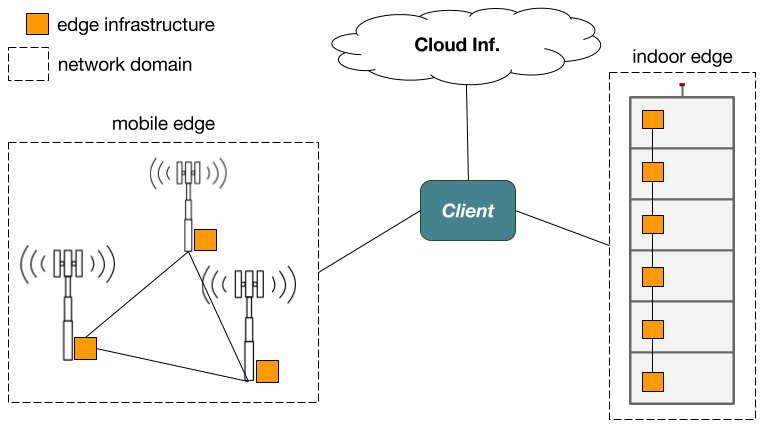
\includegraphics[width=0.5\textwidth]{figs/edge-heterogeneity.png}}
	\captionsetup[subfigure]{width=0.45\textwidth}	
	\hfill
	\subfloat[Computational resources abstracted under different edge domains; a mobile client within connection range to edge domains A and B through access points A and B\label{fig:edge-domain-client}] {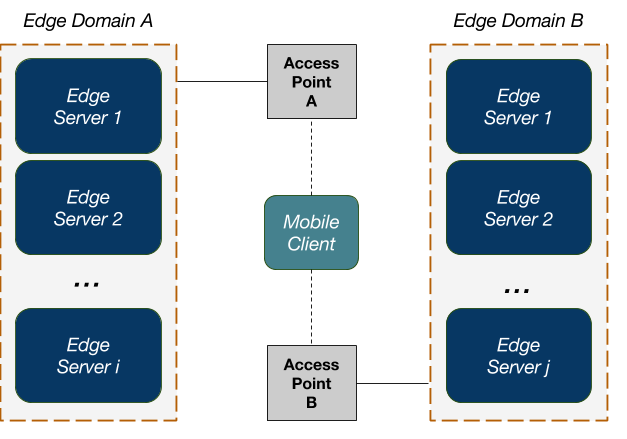
\includegraphics[width=0.45\textwidth]{figs/edge-domain-client.png}}
	\hfill\null
	\caption{Edge heterogeneity}\label{fig:1}
\end{figure}

%In addition, different kinds of edge infrastructure (e.g., more powerful servers or single board computers) or the same kind of edge infrastructure at different contexts (e.g., the number of clients in an area is too high in one region and low in another) may fit better with different policies for edge resources usage. 

\subsubsection{Client Awareness and Domain Selection}

An important aspect of edge computing consists of how edge services should be discovered and consumed by clients. 

Today, networking protocols and technologies are the main responsibles for allowing client applications to access cloud services in a transparent way. For this, clients access cloud services by means of well-known Internet names. The datacenters hosting cloud services are, at best, coarsely distributed among continents, countries, or broader regions. 
%In these cases, services names are mapped to either the servers hosting them or to intermediate components (e.g., traffic managers) responsible for transparently routing client requests to datacenters covering their area. 
In contrast, in a fine grained geographical distribution of edge computing infrastructure, a similar transparency may not be possible. 

%In particular, two scenarios of edge computing are possible: 1) edge servers are part of the telecommunications infrastructure (e.g., they are located at cellular base stations); 2) edge servers are part of conventional infrastructure  (e.g., they are located at malls, concert halls, stadiums, office buildings, parks, etc). 
%
%In the first kind of scenario, which correspond to MEC, networking technology could be employed to make the decision of using edge or cloud infrastructure transparent for the client. For instance, active components at the base stations could divert the traffic coming from clients connected to that base station to local edge servers whenever the requested services are available or to the cloud otherwise~\cite{MEC_ROUTING}. 
%
%Analogously, the second kind of scenario would require local network infrastructure components like access points and routers to actively divert the traffic from clients to edge servers in that location upon availability or to the cloud otherwise.
%
%In both cases, clients requests would be transparently handled by either edge or cloud servers, with infrastructure components responsible for taking the edge-or-cloud decision. However, in the event of both types of edge infrastructure to coexist, the client would have to participate of an edge-or-edge kind of decision.

First, because clients can switch from one network to the other at their discretion or make simultaneous use of different connections. For instance, once inside a building with some local edge servers accessible through Wi-Fi direct, the client may still decide for the edge servers available at the cellular base station it is connected (e.g., through 5G~\footnote{Fifth generation of broadband cellular technology}). 

Second, because it is unlikely that edge domains from different providers or types will be able to coordinate and decide which one will serve a given client request. For instance, at a given moment, a client device may be in contact with both MEC and indoor edge domains. If both can provide the same services, but are unable to communicate and coordinate, it is up to the client to make this decision.



%As such, whereas independent edge servers would not see each other, the client would be able to see them and decide which one suits it the best.

%In addition to the client participation in a edge-or-edge kind of decision, there is an argument in favor of giving the client also the responsibility for the edge-or-cloud type of decision: mobility. 

Finally, as mobile clients can enter or exit a given area, their connectivity with a given edge domain may be lost. The less time a mobile client remains connected to an edge domain, the lower the chances of loosing connection before it is still processing that client's request. Thus, if services are not currently available at local edge servers, clients should perform direct requests to the cloud instead of having their request forwarded by the edge network components. 

%\begin{figure}[tbp]
%	\centering
%	\captionsetup[subfigure]{width=0.5\textwidth}	
%	\null\hfill
%	\subfloat[Heterogeneus and indpendent types of edge domains (mobile and indoor) in range of communication with a client device\label{fig:edge-heterogeneity}]{ 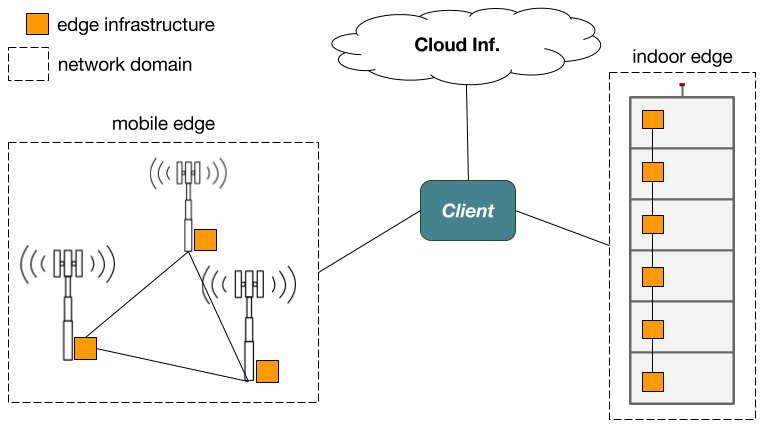
\includegraphics[width=0.5\textwidth]{figs/edge-heterogeneity.png}}
%	\captionsetup[subfigure]{width=0.45\textwidth}	
%	\hfill
%	\subfloat[In the case no edge service is available, client performs direct requests to the cloud and eliminate the dependency with intermediary edge domain infrastructure\label{fig:domain-selection}] {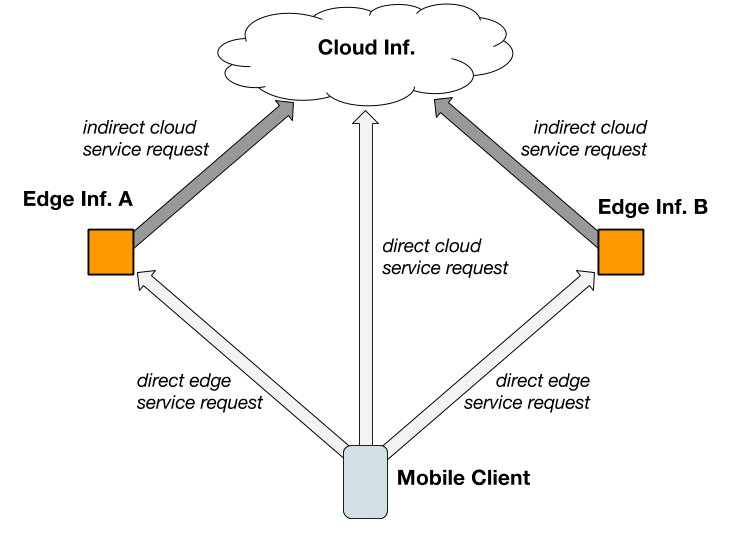
\includegraphics[width=0.45\textwidth]{figs/domain-selection.png}}
%	\hfill\null
%	\caption{Edge heterogeneity and client awareness}\label{fig:no-label-here}
%\end{figure}

Thus, the following requirements have been elicited for the discovery and selection of different computational resources:


\begin{itemize}

	\stepcounter{req_count}
	\item Edge infrastructure must be discoverable by clients (\textbf{R\arabic{req_count}}); and

	\stepcounter{req_count}
	\item Clients should have the control over which domain should be used based on its requirements and the status of edge/cloud alternatives (\textbf{R\arabic{req_count}})

\end{itemize}

%TODO: replace R2 with: Control over forwarding from edge to cloud. Soft vs. strong constraint. Soft = I can also run on cloud if needed. Strong = Never go to cloud.

\subsubsection{Client Heterogeneity}

Client applications may significantly differ in terms of the QoS they require from service providers. For example, autonomous vehicles may eventually rely on edge services for low-latency operations. An autonomous vehicle entering a given region for the first time is unlikely to be waiting until the edge servers covering that region become ready for providing the service the vehicle requires. 

Conversely, users of an augmented reality application could eventually wait for a setup time whenever the edge domain nearby are not ready. In both cases, low-latency is an important requirement. However, the later type of application could afford a setup delay which the first could not. Accordingly:

\begin{itemize}
	\stepcounter{req_count}
	\item The unified model should enable the co-existence of applications requiring different QoS levels (\textbf{R\arabic{req_count}}); and
	
	\stepcounter{req_count}
	\item The priority of the usage of edge computational resources must be in accordance with the application category and its QoS requirements (\textbf{R\arabic{req_count}})
\end{itemize}


\subsubsection{Efficiency}

Another fundamental aspect of edge computing consists of how its highly distributed computational resources should be provided and consumed.

In cloud IaaS, the infrastructure responsible for hosting and performing services is abstracted away from client applications through virtualization and more recently containerization technologies~\cite{}. In particular, the horizontal scalability provided by virtually unlimited cloud resources enables the optimization of cloud services availability, i.e., it allows these services to remain accessible and operational independently of the number of requests.

%The elasticity of cloud datacenters is enabled by its horizontal scalability, in which virtual machines or containers can be instantiated in new virtually unlimited physical resources. 


%...in which backend applications are deployed to virtual machines and/or containers....

A direct replication of cloud computing IaaS model with edge computing infrastructure would not be possible. Instead, the fine grained nature of edge computing suggests the need of a different approach for the provisioning and usage of its computational resources. 

First, because it would mean that applications would have to be deployed to each edge domain, even when there are no clients in the area been served. Such an \textit{always-available} model suites well with services covering either large or dense areas in which requests are always expected. But an alternative a more efficient provisioning model should be adopted otherwise.

Second, because it is unlikely that a significant number of applications could be simultaneously hosted by edge servers using technologies such as virtualization and containerization. 

Even if containers can be allocated faster than virtual machines~\cite{Giovanni?}, at its best, a minimum amount of resources still needs to be allocated to always-deployed containers. Thus, the scalability of edge computing in terms of number of simultaneous applications would be limited. 
	
In addition to runtime resource allocation, the multiplicity of edge domain and their limitations also suggests that a priori acquisition of different applications assets to all domains would impose unnecessary burden. Even if storage is more abundant if compared to runtime resources, a proactive and indiscriminate acquisition could compromise the scalability of edge computing.

\noindent Given the considerations above, 
%the provisioning of edge infrastructure as a service can not simply mimic the model of IaaS employed with cloud computing. Accordingly, 
the following requirement have been defined:

\begin{itemize}

	\stepcounter{req_count}
	\item The allocation of runtime resources should be opportunistic, without minimum preallocation per application, unless justified otherwise (\textbf{R\arabic{req_count}}); and
	
	\stepcounter{req_count}
	\item The acquisition of application assets should be opportunistic, unless justified otherwise (\textbf{R\arabic{req_count}})

\end{itemize} 

The fulfillment of the above requirements would leverage the potential of edge computing by optimizing the usage of its resources and consequently allowing a larger number of client applications to share the costs of edge infrastructure. Moreover, the resulting unified model would work as an extension of today’s cloud IaaS with the twofold purpose of enabling applications with low latency requirements to make use of edge infrastructure and to augment the computational power of mobile devices through mobile to edge computation offloading. 